\section*{Summary}


The focus of our team's work is on using explainable machine learning, clinical pathway simulation, and geographic modelling, applied to national clinical audit data to identify between-hospital variation in clinical decision-making and processes, and understanding the impact of that variation on patients. Our work is in collaboration with the Sentinel National Stroke Audit Programme, and focuses mostly on the emergency stroke pathway, but is applicable across other clinical areas.

We would like to enhance our methodology by adding causal analysis methods to support the explainable machine learning. This would include a literature review, but we expect it to include methods such as:

\begin{markdown}
* Clinical Trial Emulation
* Bayesian networks
* Causal Inference Machine Learning
* Instrumental Variable Analysis
\end{markdown}

As no method is perfect we wish to be able to develop a range of causal models to allow triangulation of results, and identify the best methods to incorporate into our integratred modelling and data science approach.

This enhanced methodology has potential immediate uses that will benefit patients and the NHS:

* We are working with the national stroke audit to help build machine learning into their national audit outputs, especially on unnecessary variation in use of clot-bust treatments in stroke. We are working with NHS-England to provide this analysis to new communities of practice in stroke. We have identified that a majority of the variation comes from differences in clinical decision-making rather than in differences in local patient populations. This is a NIHR-funded project \footnote{https://fundingawards.nihr.ac.uk/award/NIHR134326}. The methodological development will enhance the breadth and depth of that work, helping to identify and isolate causal relationships. Improving use of clot-busting drugs will benefit patients (and should reduce inpatient length of stay).

* We are working on stroke projects focussing on the pre-hospital pathway \footnote{https://fundingawards.nihr.ac.uk/award/NIHR202361} and the use of mobile stroke units \footnote{https://fundingawards.nihr.ac.uk/award/NIHR153982 (page due to go live)}. The methodological development above will add value to these, and other similar, projects. For example, it has previously been assumed that outcome from hemorrhagic stroke (the 20\% of strokes that are caused by a bleed rather than a clot) is independent of ambulance travel time, but some recent clinical trials on taking stroke patients further, to a hospital with more capabilities for stokes caused by clots, have suggested this may not be true. Using methods such as clinical trial emulation and our large database of stroke data we will have the potential to enhance our pre-hospital stroke care model to better model outcomes of haemorrhagic strokes with alternative pre-hospital pathways.

During this project we will hold stakeholder workshops, to obtain feedback on the work. This will use our existing stakeholder network across thr Sentinel Stroke National Audit, Integrated Stroke Delivery Networks (ISDN) and Integrated Care Systems (ICS). We will also hold regular meetings with our stroke Patient and Carer Involvement group.

In addition to development of the methodology, this project will be used to develop the skills and capabilities of Kerry Pearn (co-PI) who will lead the project with assistance from Michael Allen (Co-PI). The stroke modelling and data science team is a stable team, funded by research grants and NHS-contracted work, and the techniques and skills developed here will find long-term use and benefit.


\begin{figure}[htbp]
\centering
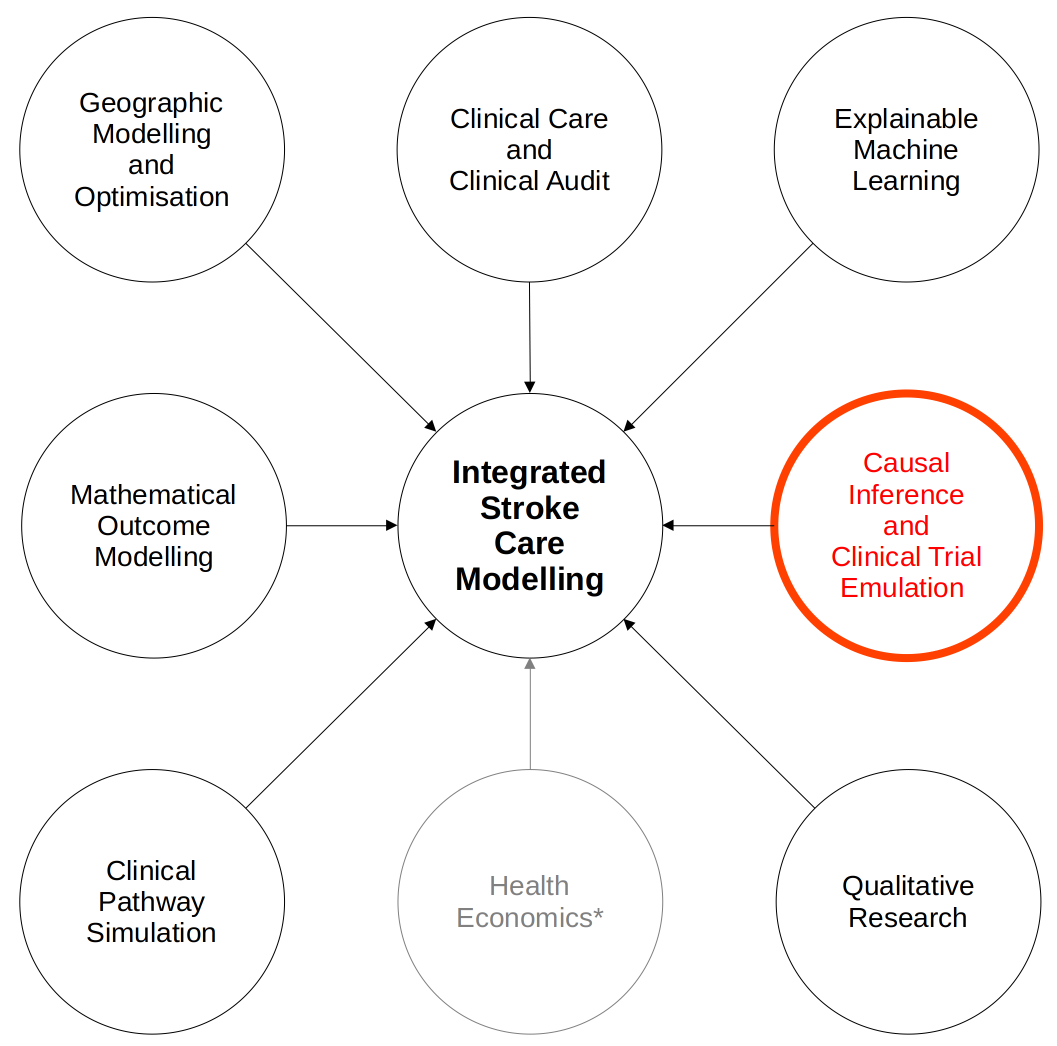
\includegraphics[width=0.6\textwidth]{./images/expertise}
\caption{How planned methodology development (red) fits in with existing team skills (black) or collaborative work (grey). All methods are fully pubslished with open code.}.
\label{fig:expertise}
\end{figure}
